\begin{surferPage}{Кумерова површ четвртог степена}
    Едуард Кумер је био први човек који је 1875. године екплицитно поставио питање о 
    максималном броју $\mu(d)$ површи четвртог степена. 
  
  Показао је да је $\mu(4)=16$. Након тога је детаљно проучавао површи четвртог степена 
  са $16$ сингуларитета.
    Посебно лепа фамилија ових површи је дата једначином:
    \[\bigl(x^2+y^2+z^2-\mu^2\bigr)^2 - \lambda
    \,y_0\,y_1\,y_2\,y_3,\]
    где је $\mu$ слободан параметар , и 
    $\lambda = \frac{3\mu^2-1}{3-\mu^2}$; $y_i$ су странице правилног тетраедра
    {\small
    $y_0=1-z-\sqrt{2}x$, \  
    $y_1=1-z+\sqrt{2}x$, \ 
    $y_2=1+z+\sqrt{2}y$, \ 
    $y_3=1+z-\sqrt{2}y$},
  како би површ била симетрична.
  Немају сви чланови ове фамилије тачно 16 реалних сингуларитета, мада већина има.
  \begin{center}
    \vspace*{-0.2cm}\hspace*{-0.2cm}
    \begin{tabular}{@{}c@{\,}c@{\,}c@{\,}c@{\,}c@{}}
      \begin{tabular}{@{}c@{}}
        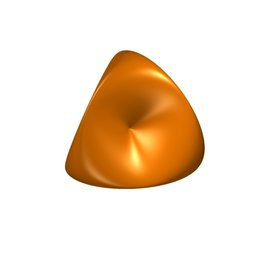
\includegraphics[height=1.4cm]{./../../common/images/kummer_0}
      \end{tabular}
      &
      \begin{tabular}{@{}c@{}}
        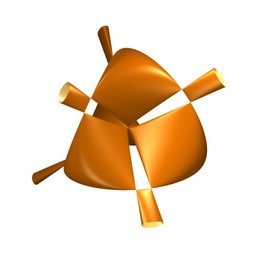
\includegraphics[height=1.4cm]{./../../common/images/kummer_1}
      \end{tabular}
      &
      \begin{tabular}{@{}c@{}}
        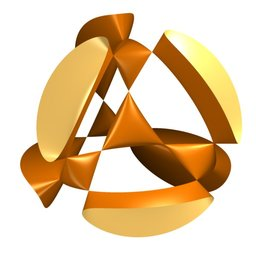
\includegraphics[height=1.4cm]{./../../common/images/kummer_2}
      \end{tabular}
      &
      \begin{tabular}{@{}c@{}}
        
\includegraphics[height=1.4cm]{./../../common/images/kummer_3}
      \end{tabular}
    \end{tabular}
  \end{center}
  \vspace{-0.2cm}  
   За неке специјалне вредности параметара, неколико сингуларитета може да се поклопи.
\end{surferPage}
